%!xelatex = 'xelatex --halt-on-error %O %S'

\documentclass{thuemp}
\usepackage{listings}
\usepackage{hyperref}
\hypersetup{hidelinks,
	colorlinks=true,
	allcolors=black,
	pdfstartview=Fit,
	breaklinks=true}
% 用来设置附录中代码的样式

\lstset{
    basicstyle          =   \sffamily,          % 基本代码风格
    keywordstyle        =   \bfseries,          % 关键字风格
    commentstyle        =   \rmfamily\itshape,  % 注释的风格,斜体
    stringstyle         =   \ttfamily,  % 字符串风格
    flexiblecolumns,                % 别问为什么,加上这个
    numbers             =   left,   % 行号的位置在左边
    showspaces          =   false,  % 是否显示空格,显示了有点乱,所以不现实了
    numberstyle         =   \zihao{-5}\ttfamily,    % 行号的样式,小五号,tt等宽字体
    showstringspaces    =   false,
    captionpos          =   t,      % 这段代码的名字所呈现的位置,t指的是top上面
    frame               =   lrtb,   % 显示边框
}

\lstdefinestyle{Python}{
    language        =   Python, % 语言选Python
    basicstyle      =   \zihao{-5}\ttfamily,
    numberstyle     =   \zihao{-5}\ttfamily,
    keywordstyle    =   \color{blue},
    keywordstyle    =   [2] \color{teal},
    stringstyle     =   \color{magenta},
    commentstyle    =   \color{red}\ttfamily,
    breaklines      =   true,   % 自动换行,建议不要写太长的行
    columns         =   fixed,  % 如果不加这一句,字间距就不固定,很丑,必须加
    basewidth       =   0.5em,
}
\begin{document}

% 标题,作者
\emptitle{面向视觉导航的认知构图与规划}
\empauthor{方桂安}{王涛老师}

% 奇数页页眉 % 请在这里写出第一作者以及论文题目
\fancyhead[CO]{{\footnotesize 方桂安: 面向视觉导航的认知构图与规划}}


%%%%%%%%%%%%%%%%%%%%%%%%%%%%%%%%%%%%%%%%%%%%%%%%%%%%%%%%%%%%%%%%
% 关键词 摘要 首页脚注
%%%%%%%%关键词
\Keyword{视觉导航, 认知图谱, 映射, 规划, 神经架构}
\twocolumn[
\begin{@twocolumnfalse}
\maketitle

%%%%%%%%摘要
\begin{empAbstract}
本次实验的目的是构建一个单或多智能体的认知导航、认知规划、认知控制仿真
算例,故我在\href{https://paperswithcode.com/}{PapersWithCode}与
\href{https://www.webofscience.com/}WebOfScience{}上查阅了诸多文献。
从中选择了这个方向并基于课堂所学认知智能知识点对该论文 \cite{2017Cognitive} \cite{2019Learning}
进行了试验和复现。在这过程中,我深入了解了认知智能的概念,并且在实验中  体会
到前沿科研方向的研究。
\end{empAbstract}

%%%%%%%%首页角注,依次为实验时间、报告时间、学号、email
\empfirstfoot{\today}{\today}{20354027}{fanggan@mail2.sysu.edu.cn}
\end{@twocolumnfalse}
]
%%%%%%%%!首页角注可能与正文重叠,请通过调整正文中第一页的\enlargethispage{-3.3cm}位置手动校准正文底部位置:
%%%%%%%%%%%%%%%%%%%%%%%%%%%%%%%%%%%%%%%%%%%%%%%%%%%%%%%%%%%%%%%%
%  正文由此开始
\wuhao 
%  分栏开始

\section{引~~言}
\enlargethispage{-3.3cm}
这篇论文介绍了一种机器人在未知环境中导航的神经(网络)架构,该架构可以学习如何从第一人称视角进行构图,并生成一组动作序列
(使机器人)到达环境中的某个目标处。其中提出的认知构图与规划器(CMP)主要基于两个关键思想:
%有序列表
\begin{itemize}
  \item 将场景构图和行为规划组合在一个统一的架构下,使得场景构图可以根据规划器的需求来驱动;
  \item 一个可以在关于世界的观察集合不完整时能够进行规划的空间记忆。
\end{itemize}

CMP 能构建一个自上而下的关于世界的可信度地图(belief map)并应用一个可
微神经网络规划器来在每一个时间步骤产生下一个动作。这种关于世界的积累的
可信度使得该智能体(agent)能够跟踪其环境中已经访问过的区域。通过实验表
明该 CMP 的表现超过了反应策略(reactive strategies)和标准的基于记忆
的架构,并且可以在全新的环境中获得良好的表现。此外,结果还表明 CMP 也能
够实现特定语义的目标,比如「go to a chair」(走到椅子那里)。

\section{背~~景}
作为人类,当我们在陌生的环境导航时,我们会将先前相似的环境的经验带
入到该环境中。我们推理自由空间,障碍和环境的拓扑结构,以常识规则和
启发式导航为指导。例如,从一个房间到另一个房间,我们必须先退出最初
的房间; 去大楼另一端的房间,走进走廊比进入会议室更容易成功; 厨房更
可能位于建筑物的开放区域而不是房间中间。本文的目标是设计一个获取这
种专业知识的学习框架,并在新环境中展示机器人导航问题。

受到这种推理的启发,已经有很多研究人员开始关注更多的端到端的基于
学习的方法,这些方法直接从像素到动作,而无需通过显式的模型或状态估
计步骤。 这些方法因此享有能够从经验中学习行为的优点。 但是,有必要
仔细设计可以捕捉任务结构的体系结构。 例如使用reactive memory
-less vanilla feed forward architectures(反应式无记忆的简单前馈神经网络)
来解决视觉导航问题。相反,有学者实验已经表明,即使智能体在它们
导航的时候以“认知地图”的形式建立了复杂的空间表征,反应式智能体依然无法
做到快捷推理。
%插入图片
\begin{figure}
  \centering
  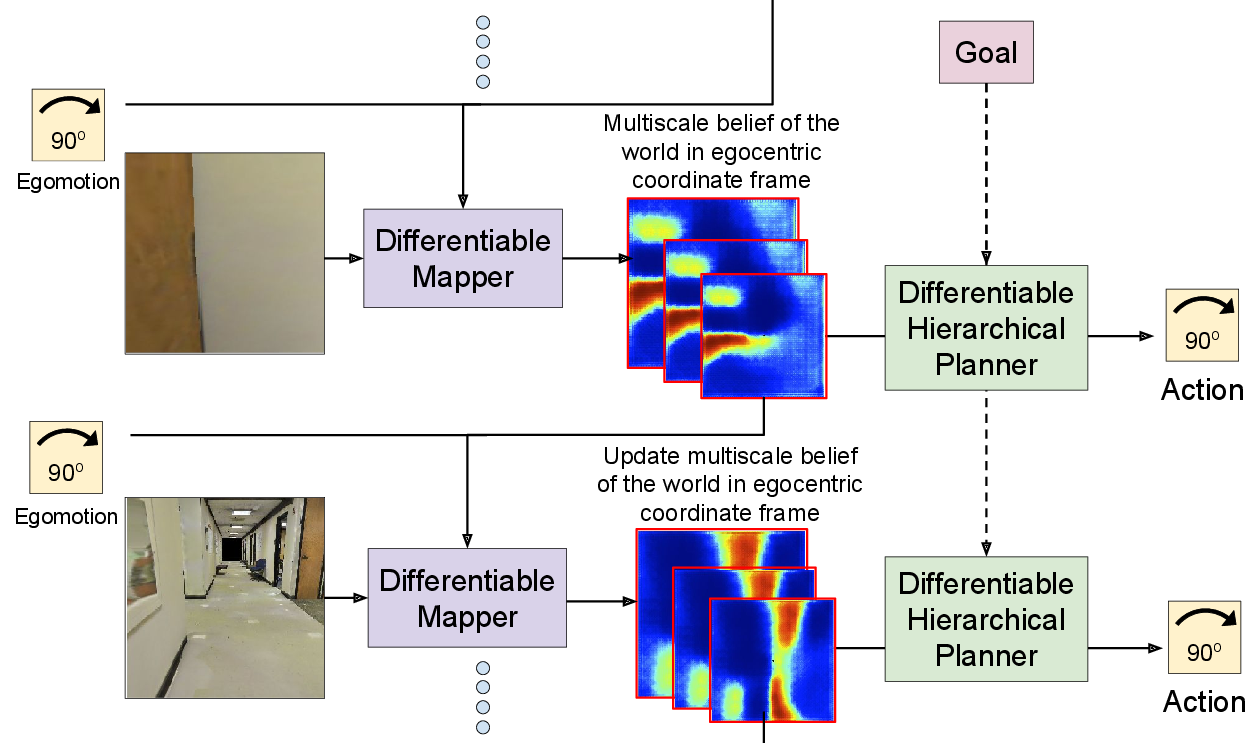
\includegraphics[width=0.5\textwidth]{image/1.png}
  \caption{Overall network architecture}
  \label{fig:CMP_architecture}
\end{figure}

这激发了作者解决视觉导航的认知构图和规划的(CMP)方法的产生\ref{fig:CMP_architecture}。
 CMP是由一种空间记忆来捕获全局的布局,以及可以规划给定的部分信息
 路径规划器。 建图器和规划器被整合到一个统一的架构中,可以通过利
 用全局的规律来训练。 该建图器融合了智能体观察到的输入视图中的信息,
 从而以自顶向下的视角产生关于世界的以度量为中心的多尺度置信度。
  规划器运用这种多层次的以世界为中心的自我中心的置信度来规划到达
  特定目标的路径并输出最佳的行动。 这个过程在每个时间步骤重复,
  以使代理人接近目标。

  在每个时间步骤,智能体从前一个时间步骤更新全局的置信度(the 
  belief of the world):
  \begin{enumerate}
    \item 使用自我运动将置信度从前一个时间步骤骤转换到当前的坐标系;
    \item 结合来自当前全局视野的信息 更新置信度。
  \end{enumerate}
  这使得智能体随着自身移动可以逐步改善全局的模式。 与之前的工作
  形成鲜明对比的是,该方法是端到端的训练,在全局上采取良好的行动。
  为此,我把这个问题作为一个学习问题进行分析,而不是单纯地计算置信度
  的更新(通过经典的运动结构),并根据观察到的第一人称视角训练
  卷积神经网络来预测更新。 我们使置信度转换和更新操作具有可区分性,
  从而实现端到端的培训。 这使得该方法能够适应实际室内场景中的统计模
  式,而不需要对绘图阶段进行任何明确的监督。

  这个方法是让人联想到经典的导航工作,也涉及到建立地图,然后在这
  些地图中规划路径,以达到预期的目标位置。 然而,该方法与传统工作
  不同之处在于以下重要方面:除了维护度量置信度的架构选择之外,
  其他一切都是从数据中学习的。 这导致了一些非常理想的特性:
  \begin{enumerate}
    \item 模型可以以任务驱动的方式学习室内环境的统计规律;
    \item 联合训练建图器和规划器使得规划器对建图器的错误更加稳健;
    \item 模型可以在新的环境中以在线方式使用,而不需要预先构建的地图。
  \end{enumerate}
\section{介~~绍}
\subsection{问题陈述}
为了研究新环境中的视觉导航问题。作者团队研究几何任务(其中任务是根据
相对于机器人当前位置的偏移量来指定的)和语义任务(其中任务是根据
到达特定对象类别来指定的)。
\subsection{方~~法}
学习的导航网络由映射器和规划器模块组成。映射器写入对应于以自我为
中心的环境地图的内在存储器,而规划器使用该存储器输出导航动作。
地图没有明确监督,而是从学习过程中自然出现。
\begin{figure}[h]
  \centering
  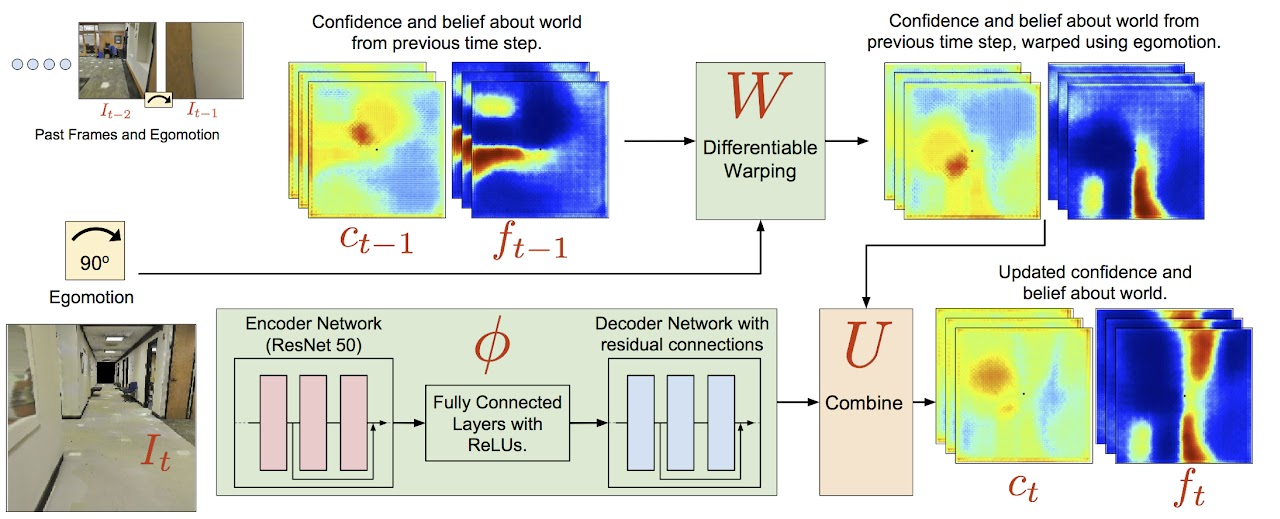
\includegraphics[width=0.5\textwidth]{image/2.jpg}
  \caption{Architecture of the mapper}
  \label{fig:map}
\end{figure}

映射器模块处理来自机器人的第一人称图像,并将观察结果整合到内在
记忆中,这对应于环境顶视图的以自我为中心的地图。映射操作不受明
确监督——映射器可以自由地将任何对规划器最有用的信息写入内存。
除了填充障碍物外,映射器还在地图中存储置信度值,这允许它通过
利用学习模式对地图中未观察到的部分进行概率预测。
\begin{figure}[h]
  \centering
  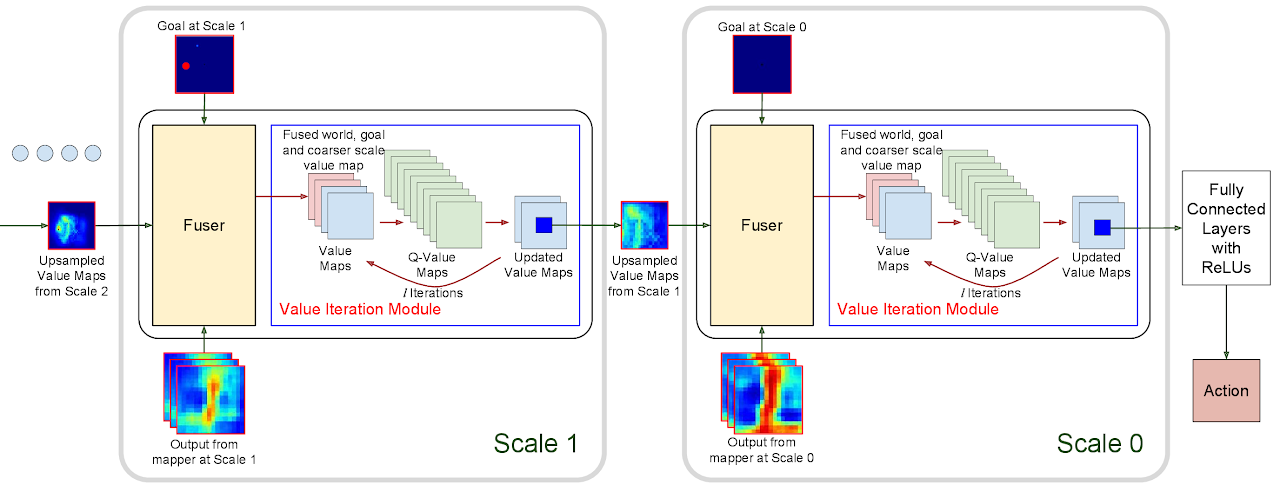
\includegraphics[width=0.5\textwidth]{image/3.png}
  \caption{Architecture of the hierarchical planner}
  \label{fig:plan}
\end{figure}

分层规划器采用映射器输出的以自我为中心的多尺度置信度,
并使用表示为卷积和通道最大池化的值迭代来输出策略。
规划器是可训练和可微的,并将梯度反向传播到映射器。规划器在问题
的多个尺度(尺度 0 是最好的尺度)上运行,从而提高规划效率。
\subsection{结~~果}
实验是在由真实世界 3D 扫描组成的静态模拟环境中进行的。
其中报告了在保留的新颖测试环境中的性能。作者报告了所提出的
方法 (CMP) 到目标的平均距离、到目标的第 75 个百分位距离和
成功率,以及反应基线和基于 LSTM 的基线。第一个表格显示几何
任务的结果,第二个表格显示语义任务的结果(转到“椅子”、“门”或“桌子”)。
\begin{figure}[h]
\centering
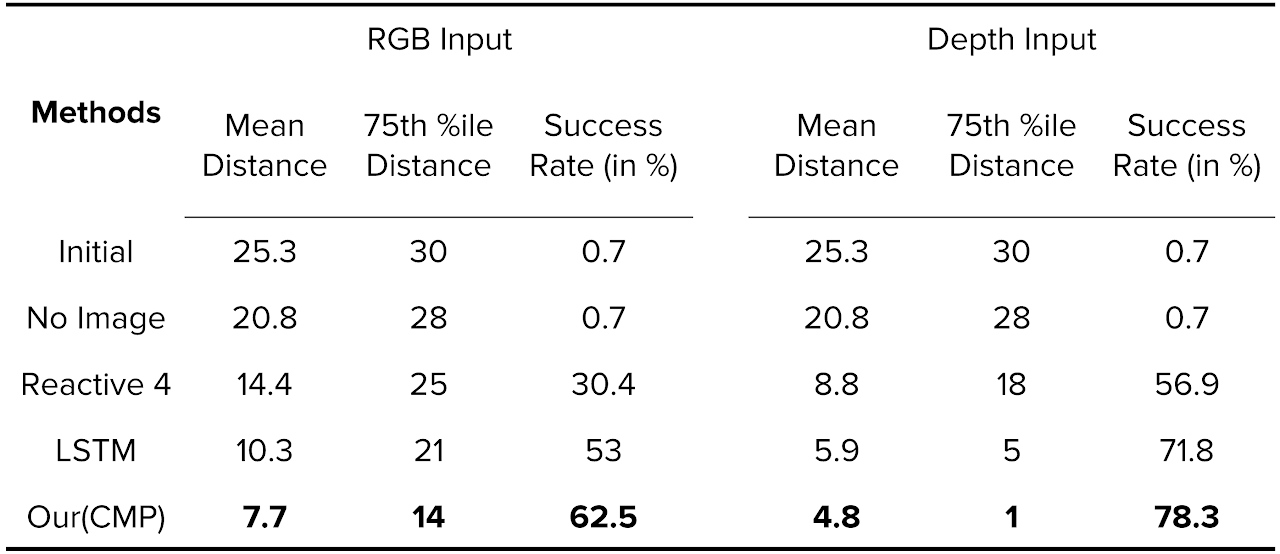
\includegraphics[width=0.5\textwidth]{image/4.png}
\end{figure}
\begin{figure}[h]
  \centering
  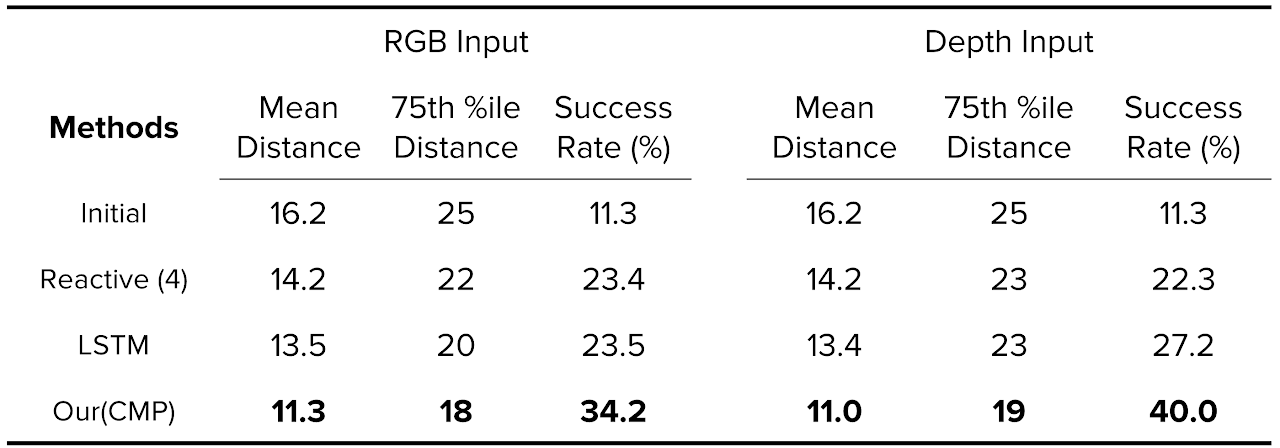
\includegraphics[width=0.5\textwidth]{image/5.png}
  \end{figure}
\section{实验复现}
\subsection{环境准备}
所有的代码都是用Python实现的,但依赖于少量的Python包和几个C库。
\begin{lstlisting}[style = Python]
  # 使用virtualenv来创建虚拟环境
  VENV_DIR=venv
  pip install virtualenv
  virtualenv $VENV_DIR
  source $VENV_DIR/bin/activate
  
  # 更新pip,并安装所需的包
  pip install --upgrade pip
  # Install simple dependencies.
  pip install -r requirements.txt

  # 打上补丁
  sh patches/apply_patches.sh
\end{lstlisting}

架构的训练用到了残差网络ResNet,它是一个深度学习模型,基于tensorflow-
1.x版本实现,不兼容tensorflow-2.x版本。故我使用以下命令安装
\begin{lstlisting}[style = Python]
  # cpu版本
  pip install tensorflow-cpu==1.15.0
  # gpu版本
  pip install tensorflow-gpu==1.15.0
\end{lstlisting}

实验使用了Swiftshader,一个基于CPU的渲染器来渲染网格。 
也可以使用其他渲染器。将`render/swiftshader\_renderer.py`中
的`SwiftshaderRenderer`做对应的修改即可。
\begin{lstlisting}[style = Python]
mkdir -p deps
git clone --recursive https://github.com/google/swiftshader.git deps/swiftshader-src
cd deps/swiftshader-src && git checkout 91da6b00584afd7dcaed66da88e2b617429b3950
git submodule update
mkdir build && cd build && cmake .. && make -j 16 libEGL libGLESv2
cd ../../../
cp deps/swiftshader-src/build/libEGL* libEGL.so.1
cp deps/swiftshader-src/build/libGLESv2* libGLESv2.so.2
\end{lstlisting}

实验使用 PyAssimp 来加载网格。 可以使用其他库来加载网格,替换
`render/swiftshader\_renderer.py` 绑定到其他库来加载网格。
\begin{lstlisting}[style = Python]
mkdir -p deps
git clone https://github.com/assimp/assimp.git deps/assimp-src
cd deps/assimp-src
git checkout 2afeddd5cb63d14bc77b53740b38a54a97d94ee8
cmake CMakeLists.txt -G 'Unix Makefiles' && make -j 16
cd port/PyAssimp && python setup.py install
cd ../../../..
cp deps/assimp-src/lib/libassimp* .
\end{lstlisting}

实验使用graph-tool进行图形处理。
\begin{lstlisting}[style = Python]
mkdir -p deps
git clone https://git.skewed.de/count0/graph-tool deps/graph-tool-src
cd deps/graph-tool-src && git checkout 178add3a571feb6666f4f119027705d95d2951ab
bash autogen.sh
./configure --disable-cairo --disable-sparsehash --prefix=$HOME/.local
make -j 16
make install
cd ../../
\end{lstlisting}
\subsection{数据准备}
从\href{http://buildingparser.stanford.edu/dataset.html}{数据集网站}\textbf{下载数据}。
\begin{enumerate}
  \item 原始网格:我们需要noXYZ文件夹中的网格。下载tar文件并将它们放在stanford\_building\_parser\_dataset\_raw文件夹中。共需下载 area\_1\_noXYZ.tar、area\_3\_noXYZ.tar、area\_5a\_noXYZ.tar、 area\_5b\_noXYZ.tar,其中area\_6\_noXYZ.tar用于训练, area\_4\_noXYZ.tar用于评估。
  \item 用于设置任务的注释。我们将需要名为Stanford3dDataset\_v1.2.zip. 将文件放在目录中stanford\_building\_parser\_dataset\_raw。
\end{enumerate}

\textbf{预处理数据}:
\begin{enumerate}
  \item 使用scripts/script\_preprocess\_meshes\_S3DIS.sh提取网格。

  之后data/stanford\_building\_parser\_dataset/mesh下应该有6个文件夹area1, area3, area4, area5a, area5b, area6, 每个目录中都有纹理和 obj 文件。
  \item 用scripts/script\_preprocess\_annoations\_S3DIS.sh从 zip 文件中提取房间信息和语义 。
  
  在此之后data/stanford\_building\_parser\_dataset下应该有room-dimension和class-maps文件夹。
\end{enumerate}

\textbf{下载ImageNet预训练模型}:我们使用 ResNet-v2-50 来训练图像。对于 RGB 图像,已经在 ImageNet 上进行预训练的。对于深度图像,我们使用成对的 RGB-D 图像将 RGB 模型提取为深度图像。
两种类型都可以通过 scripts/script\_download\_init\_models.sh初始化。
\subsection{模型训练}
作者提供了图\ref{fig:pretrained_models}中的预训练模型。
\begin{figure}[h]
  \centering
  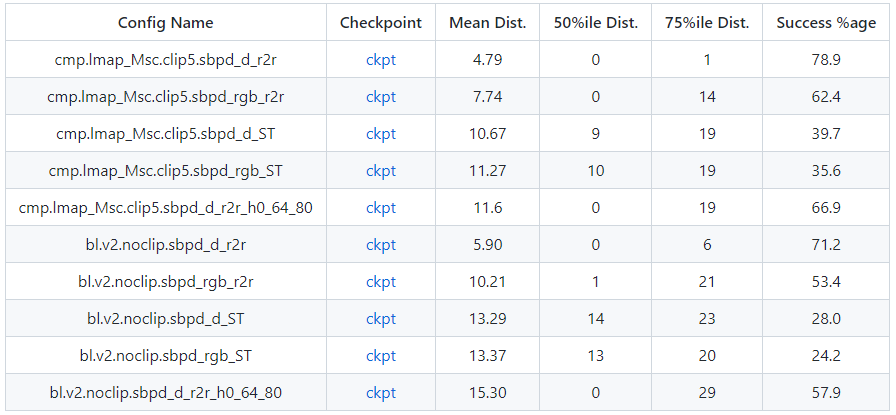
\includegraphics[width=0.5\textwidth]{image/6.png}
  \caption{预训练模型及其效果}
  \label{fig:pretrained_models}
\end{figure}
我使用了5块GTX 2080Ti GPU,16个线程来进行分布式训练。具体配置如图\ref{fig:train}所示。
\begin{figure}[h]
  \centering
  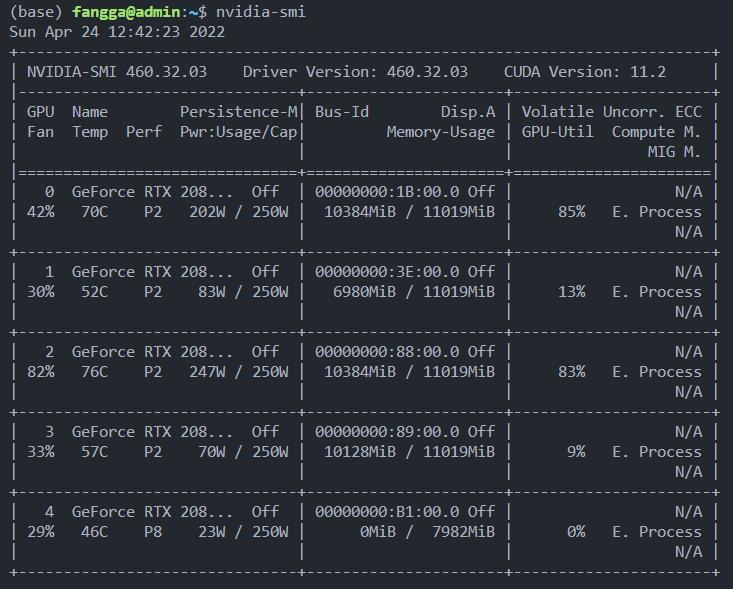
\includegraphics[width=0.5\textwidth]{image/7.jpg}
  \caption{训练配置} 
  \label{fig:train}
\end{figure}
最后使用scripts/script\_test\_pretrained\_models.sh来测试模型。
\section{复现结果}
以下图片展现了一些被构建地图的俯视图,以及智能体为实现目标所采取的行动轨迹。
%插入三张图片
\begin{figure}[h]
  \centering
  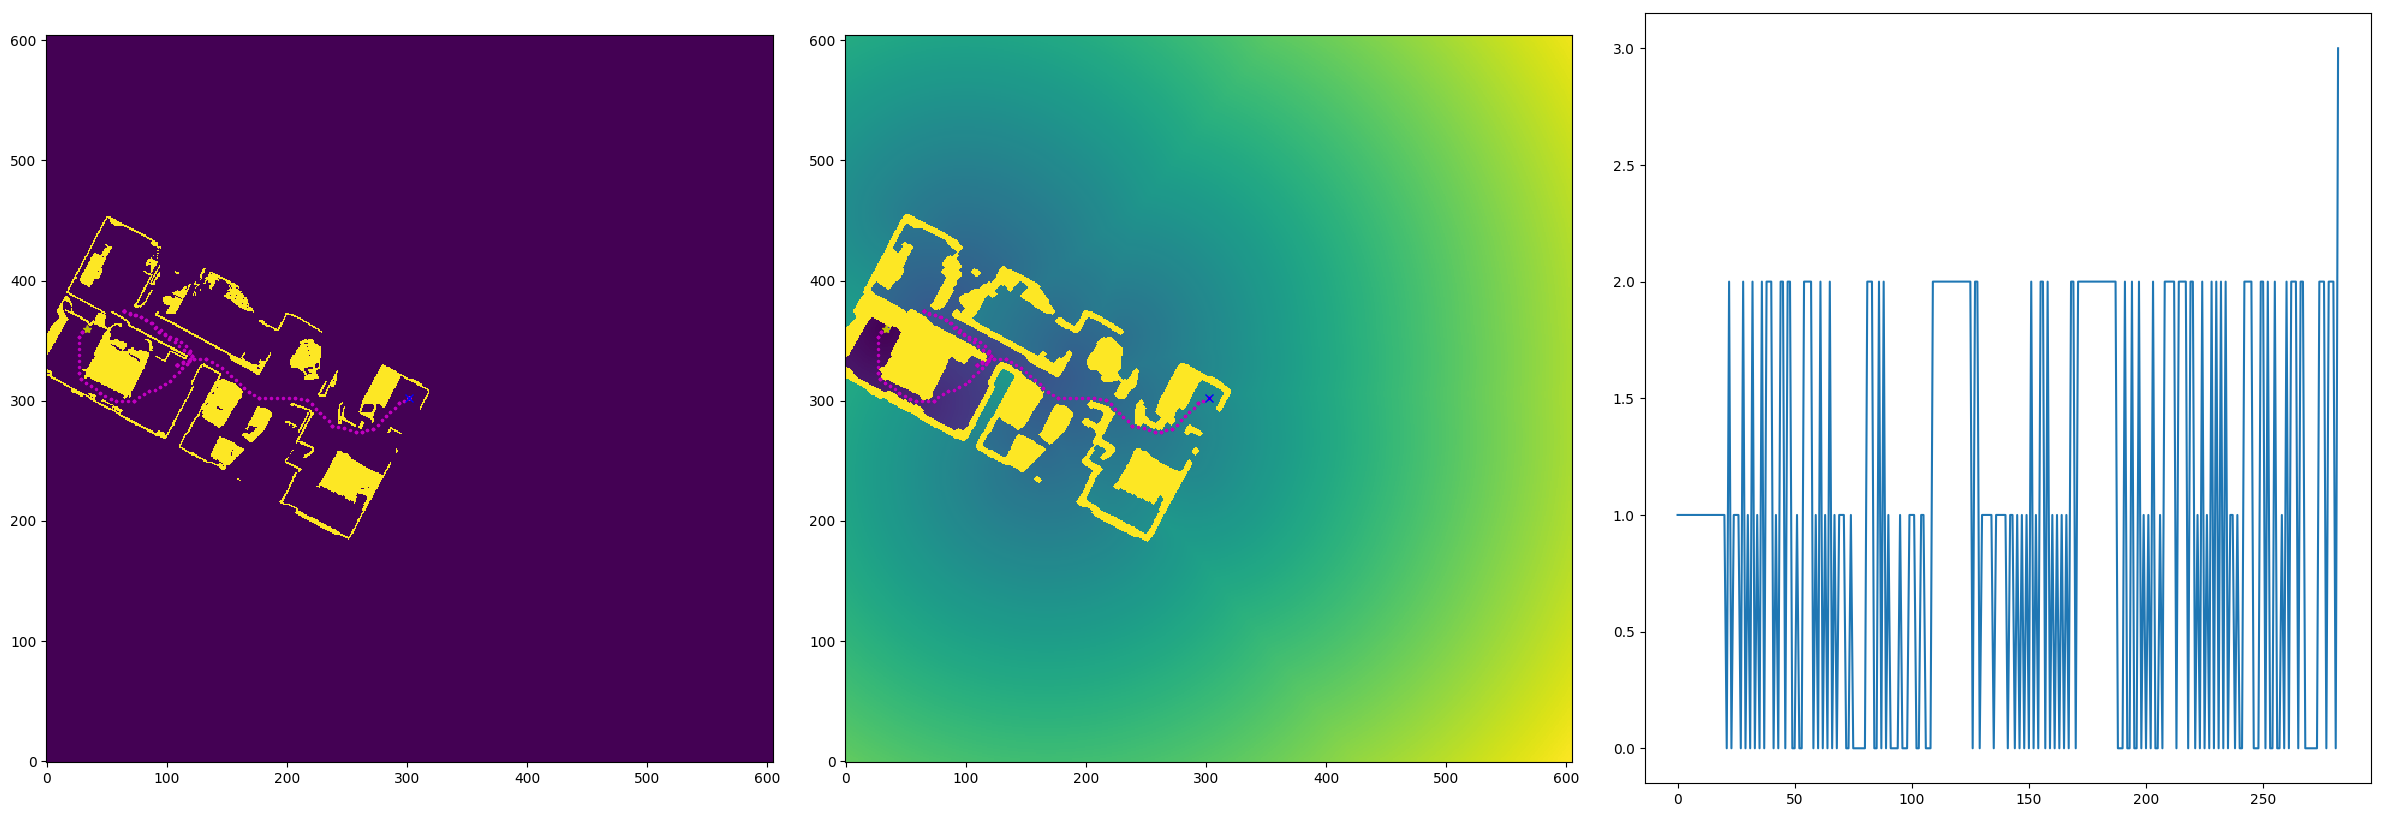
\includegraphics[width=0.5\textwidth]{image/8.png}
  \caption{结果1}
\end{figure}
\begin{figure}[h]
  \centering
  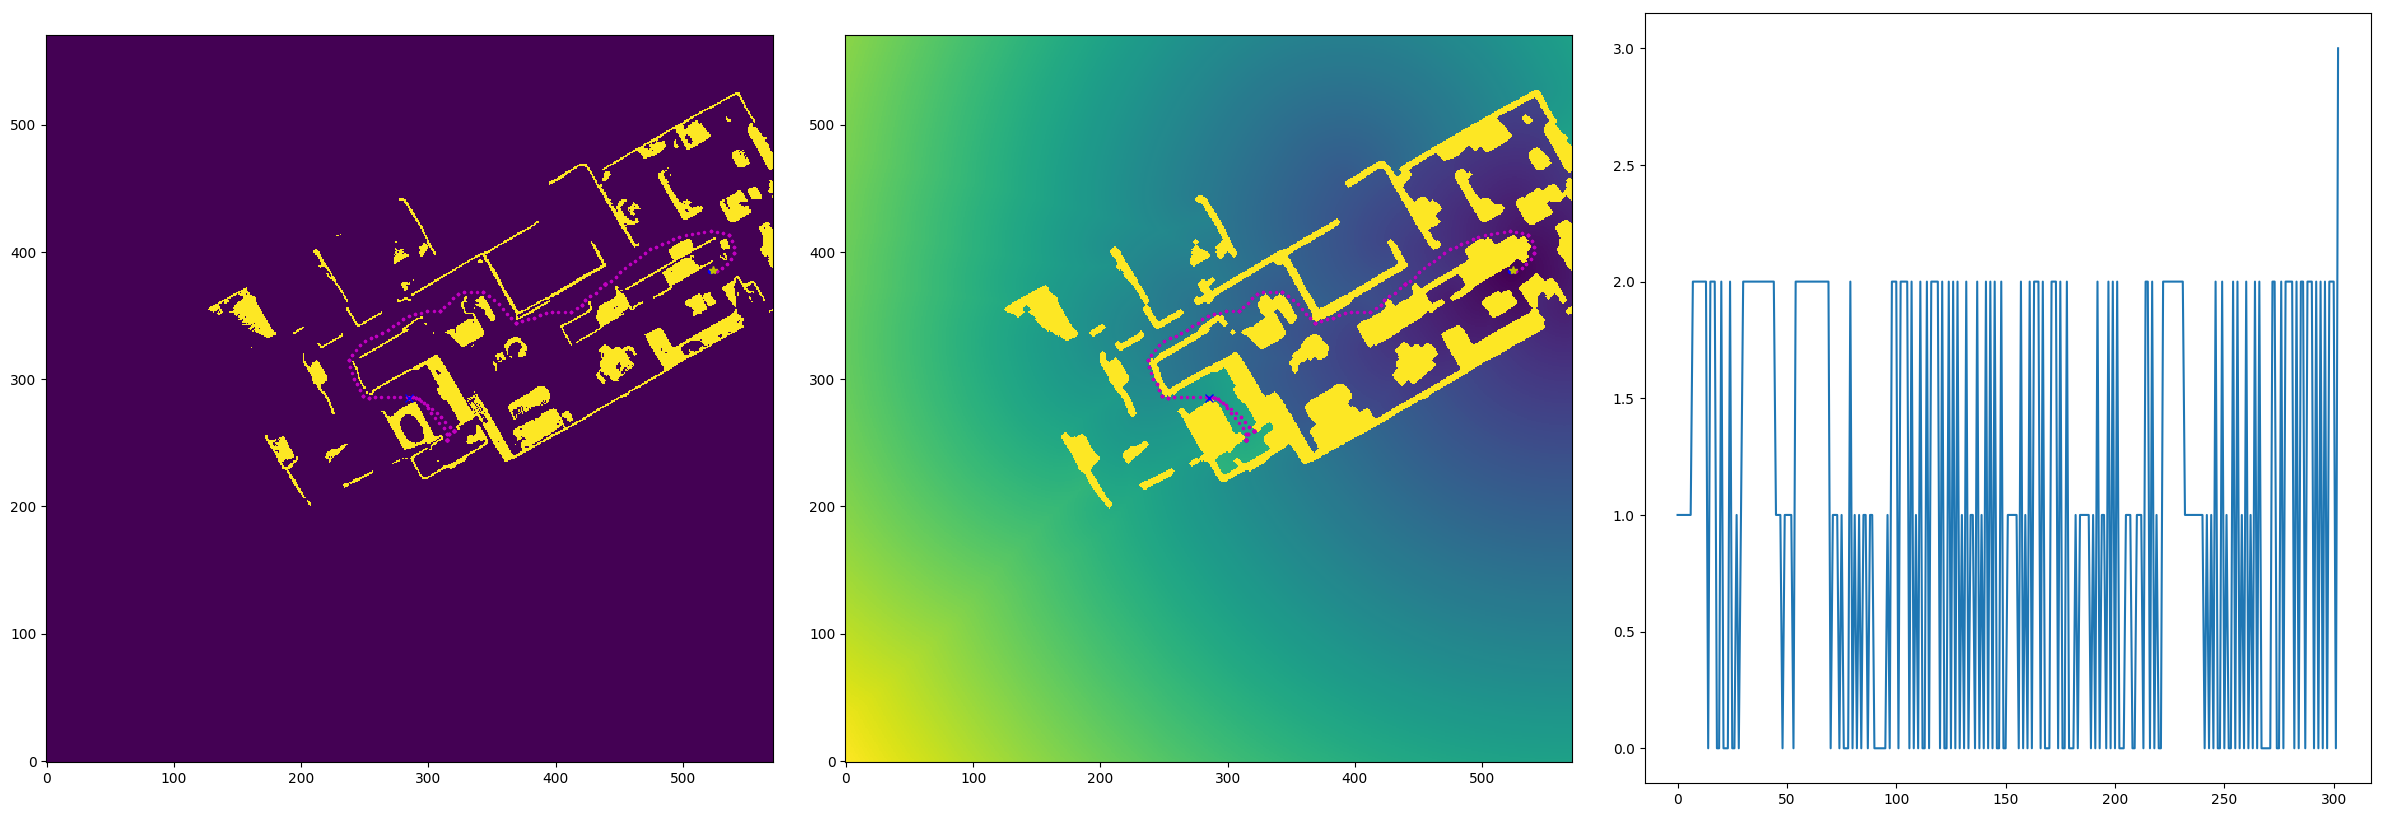
\includegraphics[width=0.5\textwidth]{image/9.png}
  \caption{结果2}
\end{figure}
\begin{figure}[h]
  \centering
  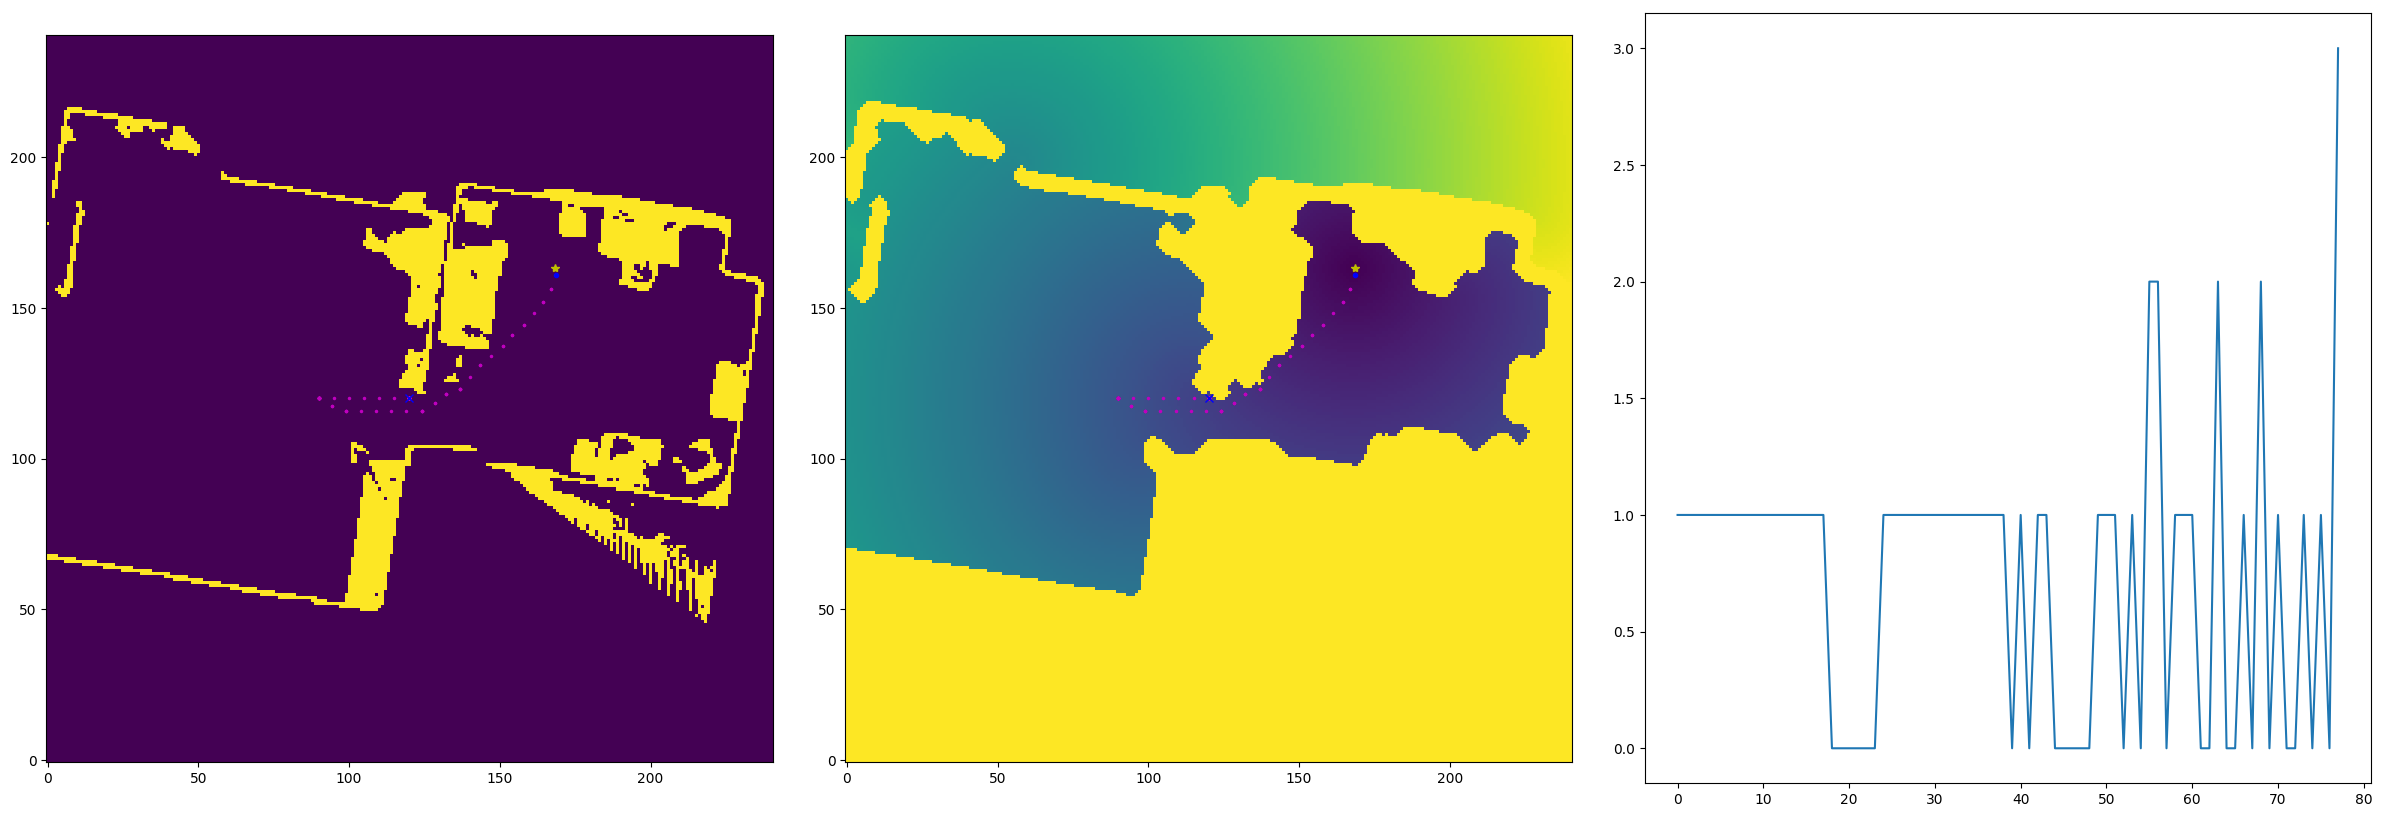
\includegraphics[width=0.5\textwidth]{image/10.png}
  \caption{结果3}
\end{figure}

在这过程中遇到了一些问题,比如:
\begin{itemize}
  \item 在拐角处卡住。这种特殊的错误很可能是由于在模拟器中处理网格缺失部分的方式或者用于确定障碍物与否的精确阈值。
  \item 建立的地图太小。我们根据目标的远近来初始化一个固定大小的地图。有可能在解决任务时,需要绕道走出地图。所以从一个大的地图开始,或者动态地调整地图的大小,可能可以解决这个问题。
  \item 碰撞恢复。摄像机直视前方,焦距为90度。这导致物体前方1.25米内的障碍物不可见,从而导致碰撞。
  我们检测这种碰撞(通过在连续的步骤中使用目标矢量),并实施恢复行为(转身并向后走1.25米),并重新扫描。
\end{itemize}
\section{感受与体会}
认知科学是对人类心智的多学科研究,包括了哲学、心理学、神经科学、计算机
科学、语言学、微电子学、教育学等。认知科学只有大约50年的发展历史,但已
经取得了长足进步,并且呈现出勃勃生机。距离理解人类心智的奥秘还有很长的
路要走,构建具备意识能力的认知科学系统具有美好的未来。
\begin{figure}
  \centering
  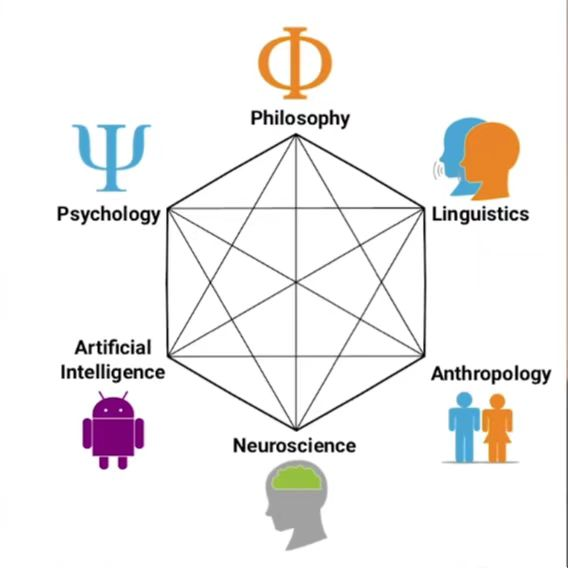
\includegraphics[width=0.5\textwidth]{image/11.jpg}
  \caption{认知科学}
\end{figure}

而人工智能(AI)就是在研究机器的认知。AI的现实目标之一,就是用计算机实现人类的智能。在研究认知现象的过程中,计算机作为一种工具也被广泛使用。计算机模拟使用模仿的手段,来研究人类的智能是如何构成的。

人工智能于一般教材中的定义领域是“智能主体(intelligent agent)的研究与设计”,智能主体指一个可以观察周遭环境并作出行动以达致目标的系统。约翰·麦卡锡于1955年的定义是“制造智能机器的科学与工程”。安德烈亚斯·卡普兰(Andreas Kaplan)和迈克尔·海恩莱因(Michael Haenlein)将人工智能定义为“系统正确解释外部数据,从这些数据中学习,并利用这些知识通过灵活适应实现特定目标和任务的能力”。 人工智能可以定义为模仿人类与人类思维相关的认知功能的机器或计算机,如学习和解决问题。

在本次试验中,我在实践中深刻体会到认知科学的魅力。通过构建机器人智能体的认知导航、认知规划和认知控制仿真,
即使该智能体还是时常“碰壁”、“迷路”,但在算法的加持下,它也在不断地修正、探索。

虽然当前的科研领域还未能制造出“真正”能推理和解决问题的智能机器,并且,这样的机器将被认为是具有知觉、有自我意识的。
但就当下的人工智能研究领域来看,研究者已大量造出“看起来”像是智能的机器,
获取相当丰硕的理论上和实质上的成果,如2009年康乃尔大学教授Hod Lipson 
和其博士研究生Michael Schmidt 研发出的 Eureqa计算机程序,只要给予一些
资料,这计算机程序自己只用几十个小时计算就推论出牛顿花费多年研究才发现
的牛顿力学公式,等于只用几十个小时就自己重新发现牛顿力学公式,
这计算机程序也能用来研究很多其他领域的科学问题上。我相信在全球众多学者
的努力下,人工智能的研究将会更加深入,未来仍充满希望。










%%%%%%%%%%%%%%%%%%%%%%%%%%%%%%%%%%%%%%%%%%%%%%%%%%%%%%%%%%%%%%%%
%  参考文献
%%%%%%%%%%%%%%%%%%%%%%%%%%%%%%%%%%%%%%%%%%%%%%%%%%%%%%%%%%%%%%%%
%  参考文献按GB/T 7714-2015《文后参考文献著录规则》的要求著录. 
%  参考文献在正文中的引用方法:\cite{bib文件条目的第一行}

\renewcommand\refname{\heiti\wuhao\centerline{参考文献}\global\def\refname{参考文献}}
\vskip 12pt

\let\OLDthebibliography\thebibliography
\renewcommand\thebibliography[1]{
  \OLDthebibliography{#1}
  \setlength{\parskip}{0pt}
  \setlength{\itemsep}{0pt plus 0.3ex}
}

{
\renewcommand{\baselinestretch}{0.9}
\liuhao
\bibliographystyle{gbt7714-numerical}
\bibliography{./TempExample}
}


\end{document}
